\hypertarget{daryl-hannah}{%
\section{Daryl Hannah}\label{daryl-hannah}}

\begin{figure}[!ht]
  \begin{adjustwidth}{-\oddsidemargin-1in}{-\rightmargin}
    \centering
    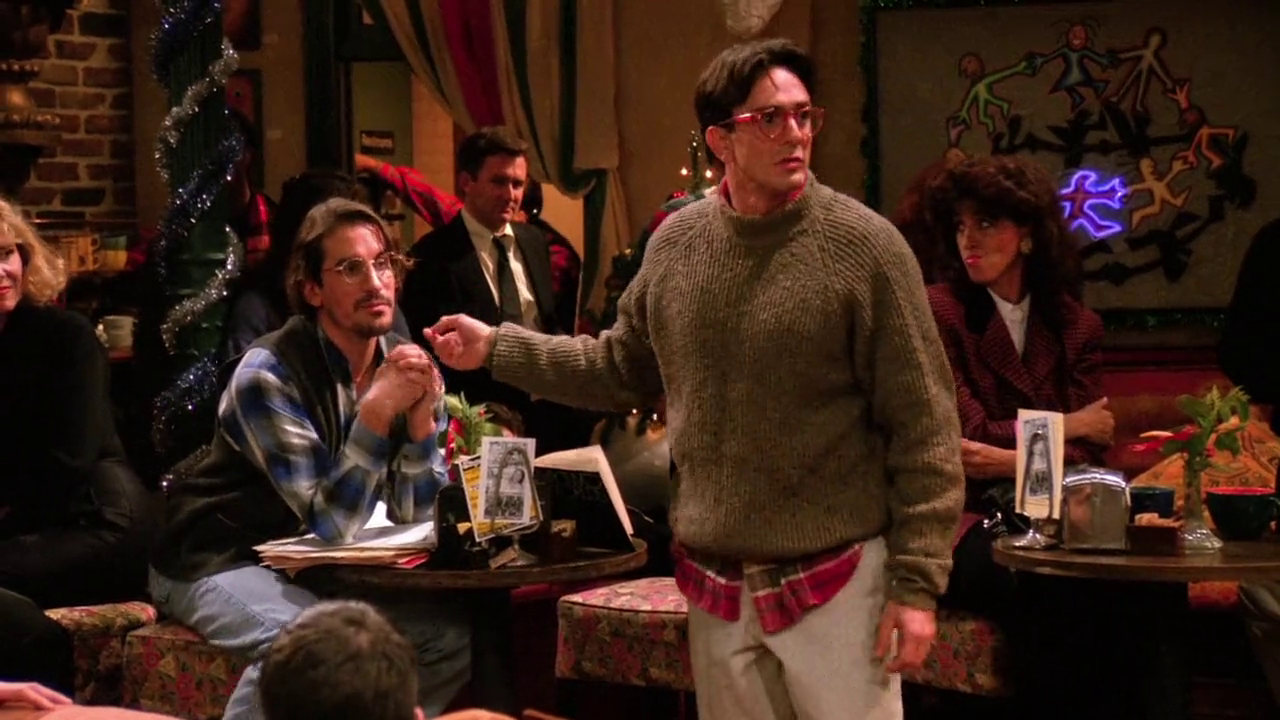
\includegraphics[trim={0 8cm 0 1cm,}, clip, width=\paperwidth]{./S01/img/10/daryl-hannah.png}
    % \caption{Daryl Hannah\label{fig:daryl-hannah}}
  \end{adjustwidth}
\end{figure}

\begin{tcolorbox}[enhanced,center upper,
    drop fuzzy shadow southeast, boxrule=0.3pt,
    lower separated=false, breakable,
    colframe=black!30!dialogoBorder,colback=white]
\begin{minipage}[c]{0.16\linewidth}
  \raisebox{\dimexpr-\height+\ht\strutbox\relax}{
    \centering 
\includegraphics[width=1.4cm]{./assets/img/david.png}
  }
   & \centering \scriptsize{David}
\end{minipage}
\hfill
\begin{minipage}[c]{0.8\linewidth}
  \textbf{- I was just saying to my friend, you were the most beautiful woman I'd ever seen. And you said Daryl Hannah...}\\
  - Estava dizendo que acho você a mulher mais linda que já vi. Ele disse que achava Daryl Hannah...
\end{minipage}

\medskip
\begin{minipage}[c]{0.16\linewidth}
  \raisebox{\dimexpr-\height+\ht\strutbox\relax}{
    \centering 
\includegraphics[width=1.4cm]{./assets/img/max.png}
  }
   & \centering \scriptsize{Max}
\end{minipage}
\hfill
\begin{minipage}[c]{0.8\linewidth}
  \textbf{- Daryl Hannah.}\\
  - Daryl Hannah.
\end{minipage}
\end{tcolorbox}

Phoebe cantava no Central Perk e logo foi interrompida pela discussão de
Max e David, sobre como David achava que Phoebe era a mulher mais bonita
que ele havia visto. Max menciona então \emph{Daryl Hannah} (1960-),
conhecida atriz, diretora e roteirista americana.\footnote{\sloppy Daryl Hannah - IMDB. \url{https://www.imdb.com/name/nm0000435/}}

David ainda menciona dois filmes em que a atriz participou. O primeiro é
\emph{Splash} (1984), uma comédia romântica onde ela protagoniza uma
sereia.\footnote{\sloppy Splash - IMDB. \url{https://www.imdb.com/title/tt0088161/}}
O outro é \emph{Wall Street} (1987), interpretando o papel de
\emph{Darien Taylor} numa história sobre o mercado de ações de Nova
York.\footnote{\sloppy Wall Street - IMDB. \url{https://www.imdb.com/title/tt0094291/}}
No Brasil, os filmes ficaram conhecidos como \emph{Splash - Uma Sereia
em Minha Vida} e \emph{Wall Street - Poder e Cobiça}, respectivamente.

\begin{figure}
  \centering
  \begin{tikzpicture}
    \node [inner sep=0pt] at (0,0) {
      
\includegraphics[width=0.6\textwidth,keepaspectratio]{./S01/img/10/splash-wall-street-posters.jpg}
    };
    \draw [white, rounded corners=\ClipSep, line width=\ClipSep]
    (current bounding box.north west) --
    (current bounding box.north east) --
    (current bounding box.south east) --
    (current bounding box.south west) -- cycle
    ;
    \end{tikzpicture}
    \caption{Splash e Wall Street - Posters\label{fig:splash-e-wall-street-posters}}
\end{figure}

\hypertarget{an-officer-and-a-gentleman}{%
\section{An officer and a Gentleman}\label{an-officer-and-a-gentleman}}

\begin{figure}[!ht]
  \begin{adjustwidth}{-\oddsidemargin-1in}{-\rightmargin}
    \centering
    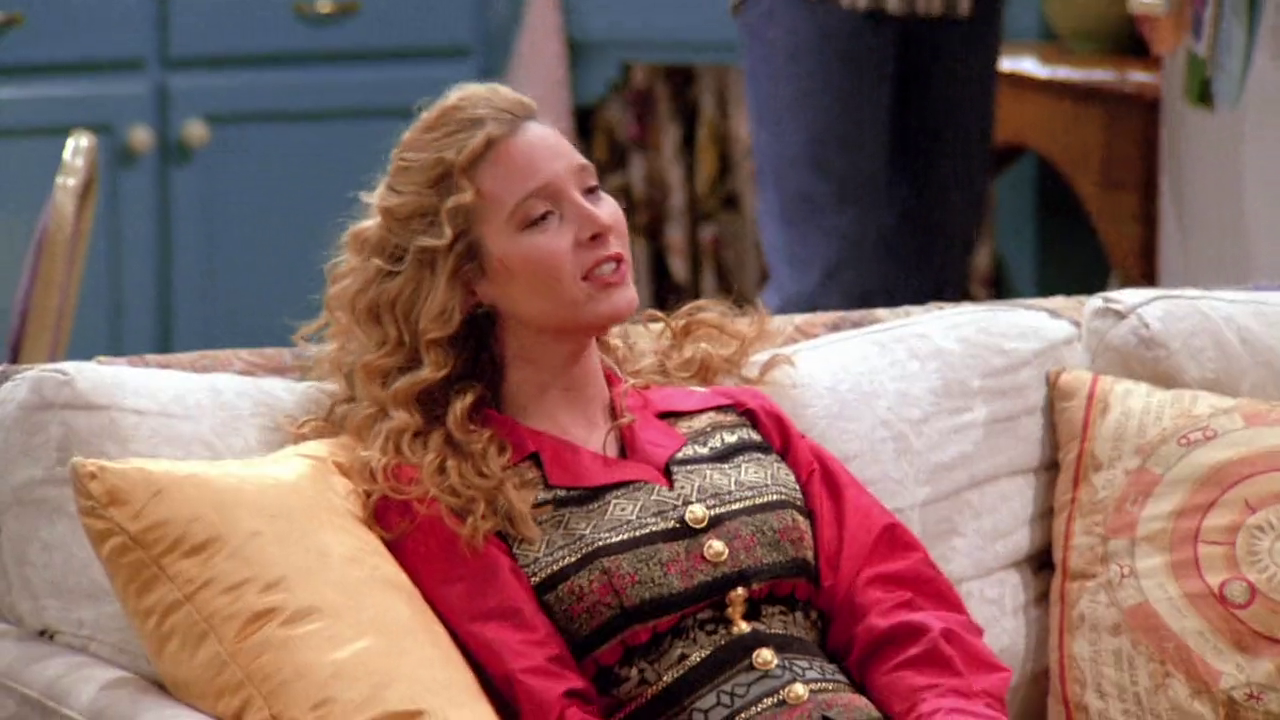
\includegraphics[trim={0 6cm 0 2cm,}, clip, width=\paperwidth]{./S01/img/10/an-officer-and-a-gentleman.png}
    % \caption{An officer and a Gentleman\label{fig:an-officer-and-a-gentleman}}
  \end{adjustwidth}
\end{figure}

\begin{tcolorbox}[enhanced,center upper,
    drop fuzzy shadow southeast, boxrule=0.3pt,
    lower separated=false, breakable,
    colframe=black!30!dialogoBorder,colback=white]
\begin{minipage}[c]{0.16\linewidth}
  \raisebox{\dimexpr-\height+\ht\strutbox\relax}{
    \centering 
\includegraphics[width=1.4cm]{./assets/img/phoebe.png}
  }
   & \centering \scriptsize{Phoebe}
\end{minipage}
\hfill
\begin{minipage}[c]{0.8\linewidth}
  \textbf{- Did you ever see An Officer and a Gentleman?}\\
  - Viu A Força do Destino?
\end{minipage}

\medskip
\begin{minipage}[c]{0.16\linewidth}
  \raisebox{\dimexpr-\height+\ht\strutbox\relax}{
    \centering 
\includegraphics[width=1.4cm]{./assets/img/monica.png}
  }
   & \centering \scriptsize{Monica}
\end{minipage}
\hfill
\begin{minipage}[c]{0.8\linewidth}
  \textbf{- Yeah.}\\
  - Sim.
\end{minipage}

\medskip
\begin{minipage}[c]{0.16\linewidth}
  \raisebox{\dimexpr-\height+\ht\strutbox\relax}{
    \centering 
\includegraphics[width=1.4cm]{./assets/img/phoebe.png}
  }
   & \centering \scriptsize{Phoebe}
\end{minipage}
\hfill
\begin{minipage}[c]{0.8\linewidth}
  \textbf{- Well, he's kind of like the guy I went to see that with.}\\
  - Ele parece o cara que viu o filme comigo.
\end{minipage}
\end{tcolorbox}

\saveparinfos
\noindent
\begin{minipage}[c]{0.5\textwidth}\useparinfo

Enquanto fala sobre David, Phoebe menciona o filme \emph{An Officer and
a Gentleman} (1982), que conta a história de \emph{Zack Mayo}
(\emph{Richard Gere}), garoto que cansado de sua vida nas Filipinas
decide entrar para Marinha, mas para isso precisa passar por um intenso
treinamento com \emph{Sgt.~Emil Foley} (\emph{Louis Gossett Jr.}). No
Brasil, o longa ficou conhecido como \emph{A Força do
Destino}.\footnote{\sloppy An Officer and a Gentleman - IMDB. \url{https://www.imdb.com/title/tt0084434/}}

\end{minipage}\hfill
\begin{minipage}[c]{0.45\textwidth}

\begin{figure}
  \centering
  \begin{tikzpicture}
    \node [inner sep=0pt] at (0,0) {
      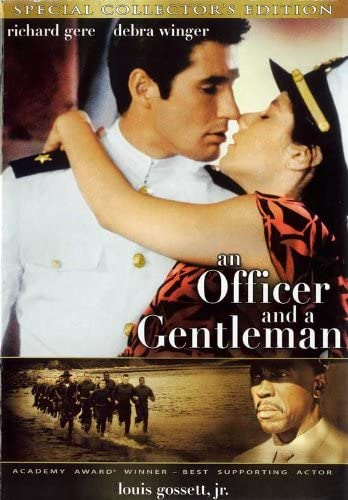
\includegraphics[width=0.7\textwidth,keepaspectratio]{./S01/img/10/an-officer-and-a-gentleman-poster.jpg}
    };
    \draw [white, rounded corners=\ClipSep, line width=\ClipSep]
    (current bounding box.north west) --
    (current bounding box.north east) --
    (current bounding box.south east) --
    (current bounding box.south west) -- cycle
    ;
    \end{tikzpicture}
    \caption{An Officer and a Gentleman - Poster\label{fig:an-officer-and-a-gentleman-poster}}
\end{figure}

\end{minipage}

\hypertarget{marvin-the-martian}{%
\section{Marvin the Martian}\label{marvin-the-martian}}

\begin{figure}[!ht]
  \begin{adjustwidth}{-\oddsidemargin-1in}{-\rightmargin}
    \centering
    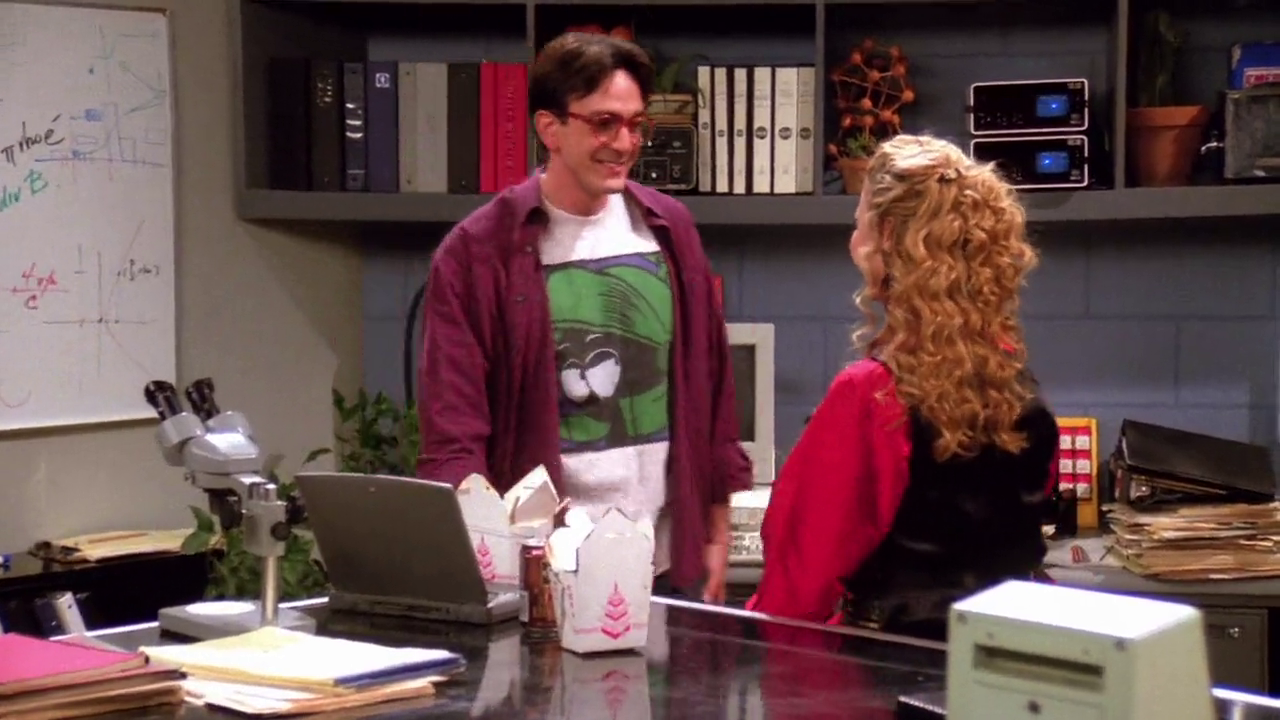
\includegraphics[trim={0 8cm 0 0cm,}, clip, width=\paperwidth]{./S01/img/10/marvin-the-martian.png}
    % \caption{Marvin the Martian\label{fig:marvin-the-martian}}
  \end{adjustwidth}
\end{figure}

\saveparinfos
\noindent
\begin{minipage}[c]{0.5\textwidth}\useparinfo

Enquanto tenta explicar a Phoebe sobre seu trabalho, David veste uma
camisa com o personagem \emph{Marvin the Martian} (1948), criatura
extraterrestre da \emph{Looney Tunes}. Aparece pela primeira vez no
episódio \emph{Haredevil Hare}.\footnote{\sloppy Marvin the Martian - Fandom Wiki. \url{https://looneytunes.fandom.com/wiki/Marvin_the_Martian}}
\footnote{\sloppy Haredevil Hare - Dailymotion. \url{https://www.dailymotion.com/video/x7sk3yr}}

\end{minipage}\hfill
\begin{minipage}[c]{0.5\textwidth}

\begin{figure}
  \centering
  \begin{tikzpicture}
    \node [inner sep=0pt] at (0,0) {
      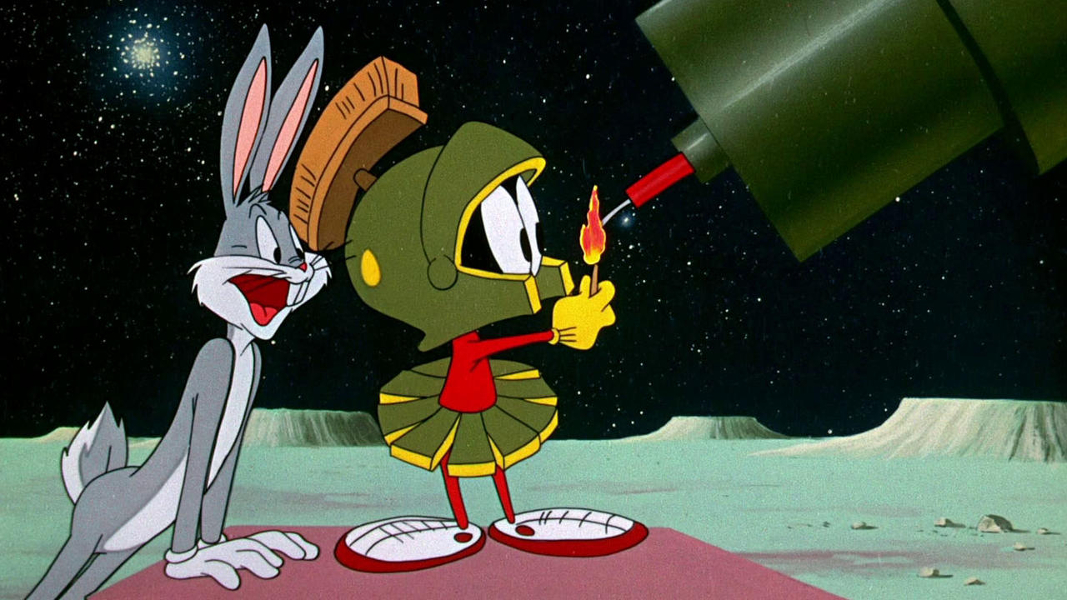
\includegraphics[width=0.8\textwidth,keepaspectratio]{./S01/img/10/haredevil-hare.jpg}
    };
    \draw [white, rounded corners=\ClipSep, line width=\ClipSep]
    (current bounding box.north west) --
    (current bounding box.north east) --
    (current bounding box.south east) --
    (current bounding box.south west) -- cycle
    ;
    \end{tikzpicture}
    \caption{Haredevil Hare\label{fig:haredevil-hare}}
\end{figure}

\end{minipage}

\hypertarget{yoko}{%
\section{Yoko}\label{yoko}}

\begin{figure}[!ht]
  \begin{adjustwidth}{-\oddsidemargin-1in}{-\rightmargin}
    \centering
    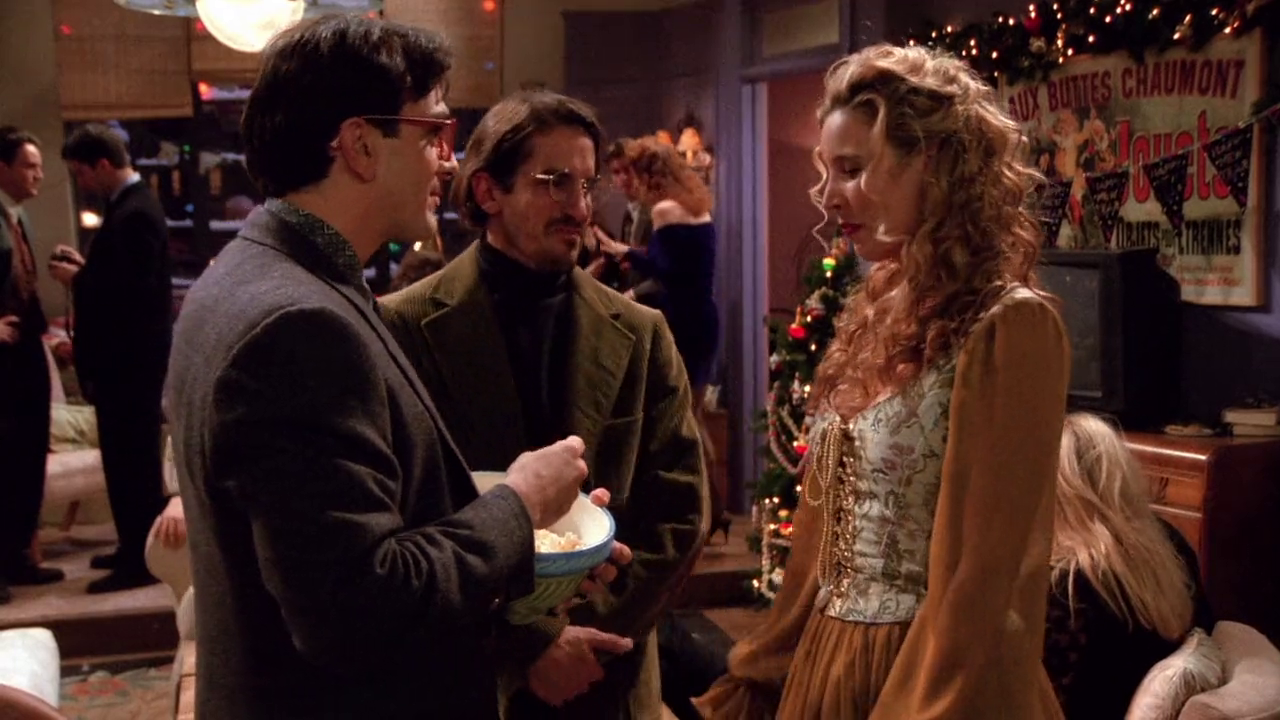
\includegraphics[trim={0 11cm 0 1cm,}, clip, width=\paperwidth]{./S01/img/10/yoko.png}
    % \caption{Yoko\label{fig:yoko}}
  \end{adjustwidth}
\end{figure}

Após cumprimentar David, seu colega de laboratório, Max chama Phoebe de
\emph{Yoko}, alusão a \emph{Yoko Ono} (1933-), que teve um
relacionamento com \emph{John Lennon} (1940-1980) e que isso teria sido
um dos motivos da seperação da banda, por volta de 1968 durante as
gravações de \emph{The White Album} (1968).\footnote{\sloppy Yoko Ono - Independent (Inglês). \url{https://bit.ly/2KG9zoM}}
\footnote{\sloppy Yoko Ono - Biography (Inglês). \url{https://www.biography.com/news/did-yoko-ono-break-up-the-beatles}}
